\subsection{Training: Selecting the Flow-Matching Recipe}
\label{sec:recipe-training}

\textbf{Explored designs.}
We ablate each training choice separately. For time sampling, we compare uniform,
logit-normal, Beta, and the Beta--uniform mixture proposed by
\citet{geffner2025proteina}. We also test
random translations in fractional coordinates, wrapping each molecule into the
unit cell by its centroid~\citep{gruver2024finetuned}. We compare $L^1$ and $L^2$ losses and vary the coordinate-to-lattice weighting in Equation~\eqref{eq:method-vfm-loss}.

We further test auxiliary supervision on periodic pair distances. Let
$\mathcal{P}=\{(i,j):i\ne j,\ d_{ij}<15\,\text{\AA}\}$, where $d_{ij}$ and
$\hat d_{ij}$ denote target and predicted minimum-image distances. We consider an
$L^1$ loss following CLARI~\citep{lo2026clari} and a periodic adaptation of
AlphaFold~3 smooth-LDDT~\citep{Abramson2024}:
\begin{equation}
    \mathcal{L}_{\mathrm{pair}}^{L^1}
    = \frac{1}{|\mathcal{P}|}\sum_{(i,j)\in\mathcal{P}}
      \left|\hat d_{ij}-d_{ij}\right|,
    \qquad
    \mathcal{L}_{\mathrm{pair}}^{\mathrm{smooth}}
    = 1-\frac{1}{4|\mathcal{P}|}\sum_{(i,j)\in\mathcal{P}}
      \sum_{\tau\in\{0.5,1,2,4\}}
      \sigma\!\left(\tau-\left|\hat d_{ij}-d_{ij}\right|\right),
    \label{eq:training-pair-losses}
\end{equation}
where $\sigma$ is the sigmoid function and distances are in angstroms.
Finally, we compare AdamW~\citep{loshchilov2019decoupled} with
Muon~\citep{liu2025muon} and evaluate raw versus EMA parameters.

\textbf{Results and selection.}
The Beta--uniform mixture outperforms pure Beta, logit-normal, and uniform time
distributions (\Cref{fig:training-recipe-summary}a). Random translation
augmentation improves $\mathrm{Sol}_C$ from $0.466$ to $0.486$, while $L^1$
substantially outperforms $L^2$ ($0.486$ vs.\ $0.407$;
\Cref{fig:training-recipe-summary}b). Increasing the coordinate-to-lattice
weight ratio improves performance from $0.412$ at $1{:}1$ to $0.486$ at
$10{:}1$, after which performance declines
(\Cref{fig:training-recipe-summary}c). Auxiliary pair supervision provides
little benefit: the best smooth-LDDT setting improves $\mathrm{Sol}_C$ by only
$0.004$ while requiring $1.37\times$ more training GPU-hours (599 vs.\ 436). Muon outperforms AdamW ($0.486$ vs.\ $0.447$), and an EMA decay of $0.9999$ outperforms both raw
weights and a decay of $0.999$ (\Cref{fig:training-recipe-summary}e--f). We
therefore select Beta--uniform time sampling, random translation augmentation,
$L^1$ endpoint regression with a $10{:}1$ coordinate-to-lattice weight ratio,
no auxiliary pair loss, Muon, and an EMA decay of $0.9999$.


\begin{figure}[!t]
  \centering
  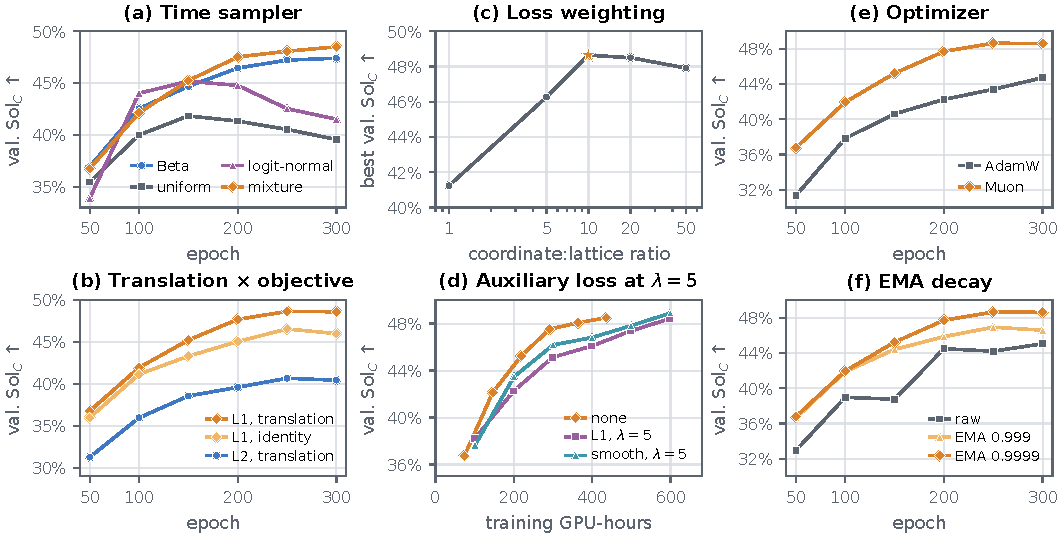
\includegraphics[width=\textwidth]{figures/generated/fig_training_recipe_summary.pdf}
  \caption{\textbf{Training recipe selection.} All panels report
    validation $\mathrm{Sol}_C$ under EDM Heun 200 with a generation budget of
    30 candidates.
    \textbf{(a)} The Beta--uniform mixture gives the strongest completed score.
    \textbf{(b)} With L1 regression, crystal translation improves the best score
    from $0.466$ to $0.486$; under translation, L1 outperforms L2
    ($0.486$ vs.\ $0.407$). \textbf{(c)} A $10{:}1$ coordinate-to-lattice
    ratio is optimal. \textbf{(d)} At $\lambda{=}5$, smooth-LDDT improves the
    best score by only $0.004$ while increasing training cost from
    436 to 599 GPU-hours. \textbf{(e)} Muon outperforms
    AdamW. \textbf{(f)} EMA decay $0.9999$ outperforms raw weights and decay
    $0.999$.}
  \label{fig:training-recipe-summary}
\end{figure}

